% !TeX program = xelatex
% !TeX encoding = UTF-8
% !TeX TXS-program:compile = txs:///xelatex | txs:///xelatex
\documentclass[aspectratio=169, table, 12pt]{beamer}
% Preamble bersama seluruh slide mata kuliah ini.
% Dipanggil dari slides/sessionXX/sessionXX.tex tepat sesudah baris
% \documentclass[aspectratio=169, table, 12pt]{beamer}
% Paket tambahan yang hanya dibutuhkan satu sesi ditulis di berkas sesi itu.

\usepackage{colortbl}
\usepackage{xcolor}
\usepackage{listings}
\usepackage{tabularx}
\usepackage{booktabs}
\usepackage{tikz}
\usepackage{pgfplots}
\pgfplotsset{compat=1.18}
\usetikzlibrary{arrows.meta, positioning, calc, fit, shapes.geometric,
	shapes.multipart, backgrounds, matrix, chains, trees}

\makeatletter
\def\input@path{{../theme/}}
\makeatother
\graphicspath{{../theme/}{../../figures/}}
\usetheme{Pradita}

\definecolor{praditagreen}{RGB}{37, 113, 71}

% Tema membuat garis tabel berwarna putih. Dikembalikan agar tabel terbaca.
\arrayrulecolor{black}
\setlength{\arrayrulewidth}{0.5pt}

\lstdefinelanguage{yaml}{
	basicstyle=\ttfamily\scriptsize,
	keywordstyle=\color{blue}\bfseries,
	commentstyle=\color{gray}\itshape,
	stringstyle=\color{red},
	showstringspaces=false,
	breaklines=true,
	frame=lines,
	numbers=none,
	backgroundcolor=\color{lightgray!10},
	tabsize=2,
	morecomment=[l]{\#}
}

\lstdefinelanguage{json}{
	basicstyle=\ttfamily\scriptsize,
	stringstyle=\color{red},
	commentstyle=\color{gray},
	breaklines=true,
	showstringspaces=false,
	tabsize=2,
	numbers=none,
	frame=lines,
	backgroundcolor=\color{lightgray!10},
	string=[s]{"}{"}
}

\lstdefinelanguage{bash}{
	keywords={},
	basicstyle=\ttfamily\scriptsize,
	ndkeywords={docker, kubectl, helm, curl, git, terraform},
	ndkeywordstyle=\color{purple}\bfseries,
	sensitive=true,
	commentstyle=\color{gray},
	numbers=none,
	breaklines=true,
	frame=lines,
	backgroundcolor=\color{lightgray!10},
	tabsize=2,
	comment=[l]{\#},
	showstringspaces=false
}

\lstdefinelanguage{http}{
	keywords={GET, POST, PUT, PATCH, DELETE, HEAD, OPTIONS, HTTP},
	basicstyle=\ttfamily\scriptsize,
	keywordstyle=\color{blue}\bfseries,
	sensitive=true,
	numbers=none,
	breaklines=true,
	frame=lines,
	backgroundcolor=\color{lightgray!10},
	tabsize=2,
	showstringspaces=false
}

\subtitle{IT40613 · Digital Platform \& API Economy}
\author{\textbf{Alfa Yohannis}}


\title{\Huge API sebagai Produk\\ \vspace{10pt} dan Ekonomi API}
\date{Pertemuan 04}

\begin{document}
\frame{\titlepage}

\begin{frame}
  \frametitle{Isi Pertemuan}
  \vspace{14pt}
  \begin{columns}[t]
    \column{0.5\textwidth}
    {\small\tableofcontents[sections={1-4}]}

    \column{0.5\textwidth}
    {\small\tableofcontents[sections={5-9}]}
  \end{columns}
\end{frame}

\begin{frame}{\hfill}
  \centering
  \Huge{\textbf{Proyek integrasinya\\sudah selesai.\\Siapa yang menjawab\\mitra besok pagi?}}
\end{frame}

\section{Tujuan dan Konteks}

\begin{frame}{{\Large Tujuan Pembelajaran}}
  \vspace{10pt}
  \begin{itemize}
    \item Menjelaskan konsep API sebagai produk dan perbedaannya dengan API sebagai proyek integrasi.
    \item Mengklasifikasikan API menurut audiensnya: privat, mitra, dan publik.
    \item Menyusun inventaris integrasi dan API yang berjalan di organisasi.
  \end{itemize}
\end{frame}

\begin{frame}{{\Large Masukan Bab 3: Tiga Sambungan Terlemah}}
  \vspace{10pt}
  \begin{itemize}
    \item 1.100 pemeriksaan per bulan dari 3 laboratorium: surel, lalu diketik ulang.
    \item 7.800 klaim per bulan ke 9 portal asuransi: 468 ditolak karena format.
    \item 36 rekap per bulan bagi perusahaan klien: disusun manual empat hari kerja.
    \item Ketiganya calon pertama API mitra.
    \item Angka berawalan ``Misalkan'' adalah asumsi latihan. Hasilnya masuk tonggak C2.
  \end{itemize}
\end{frame}

\begin{frame}{{\Large Diagram Konsep Bab 4}}
  \centering
  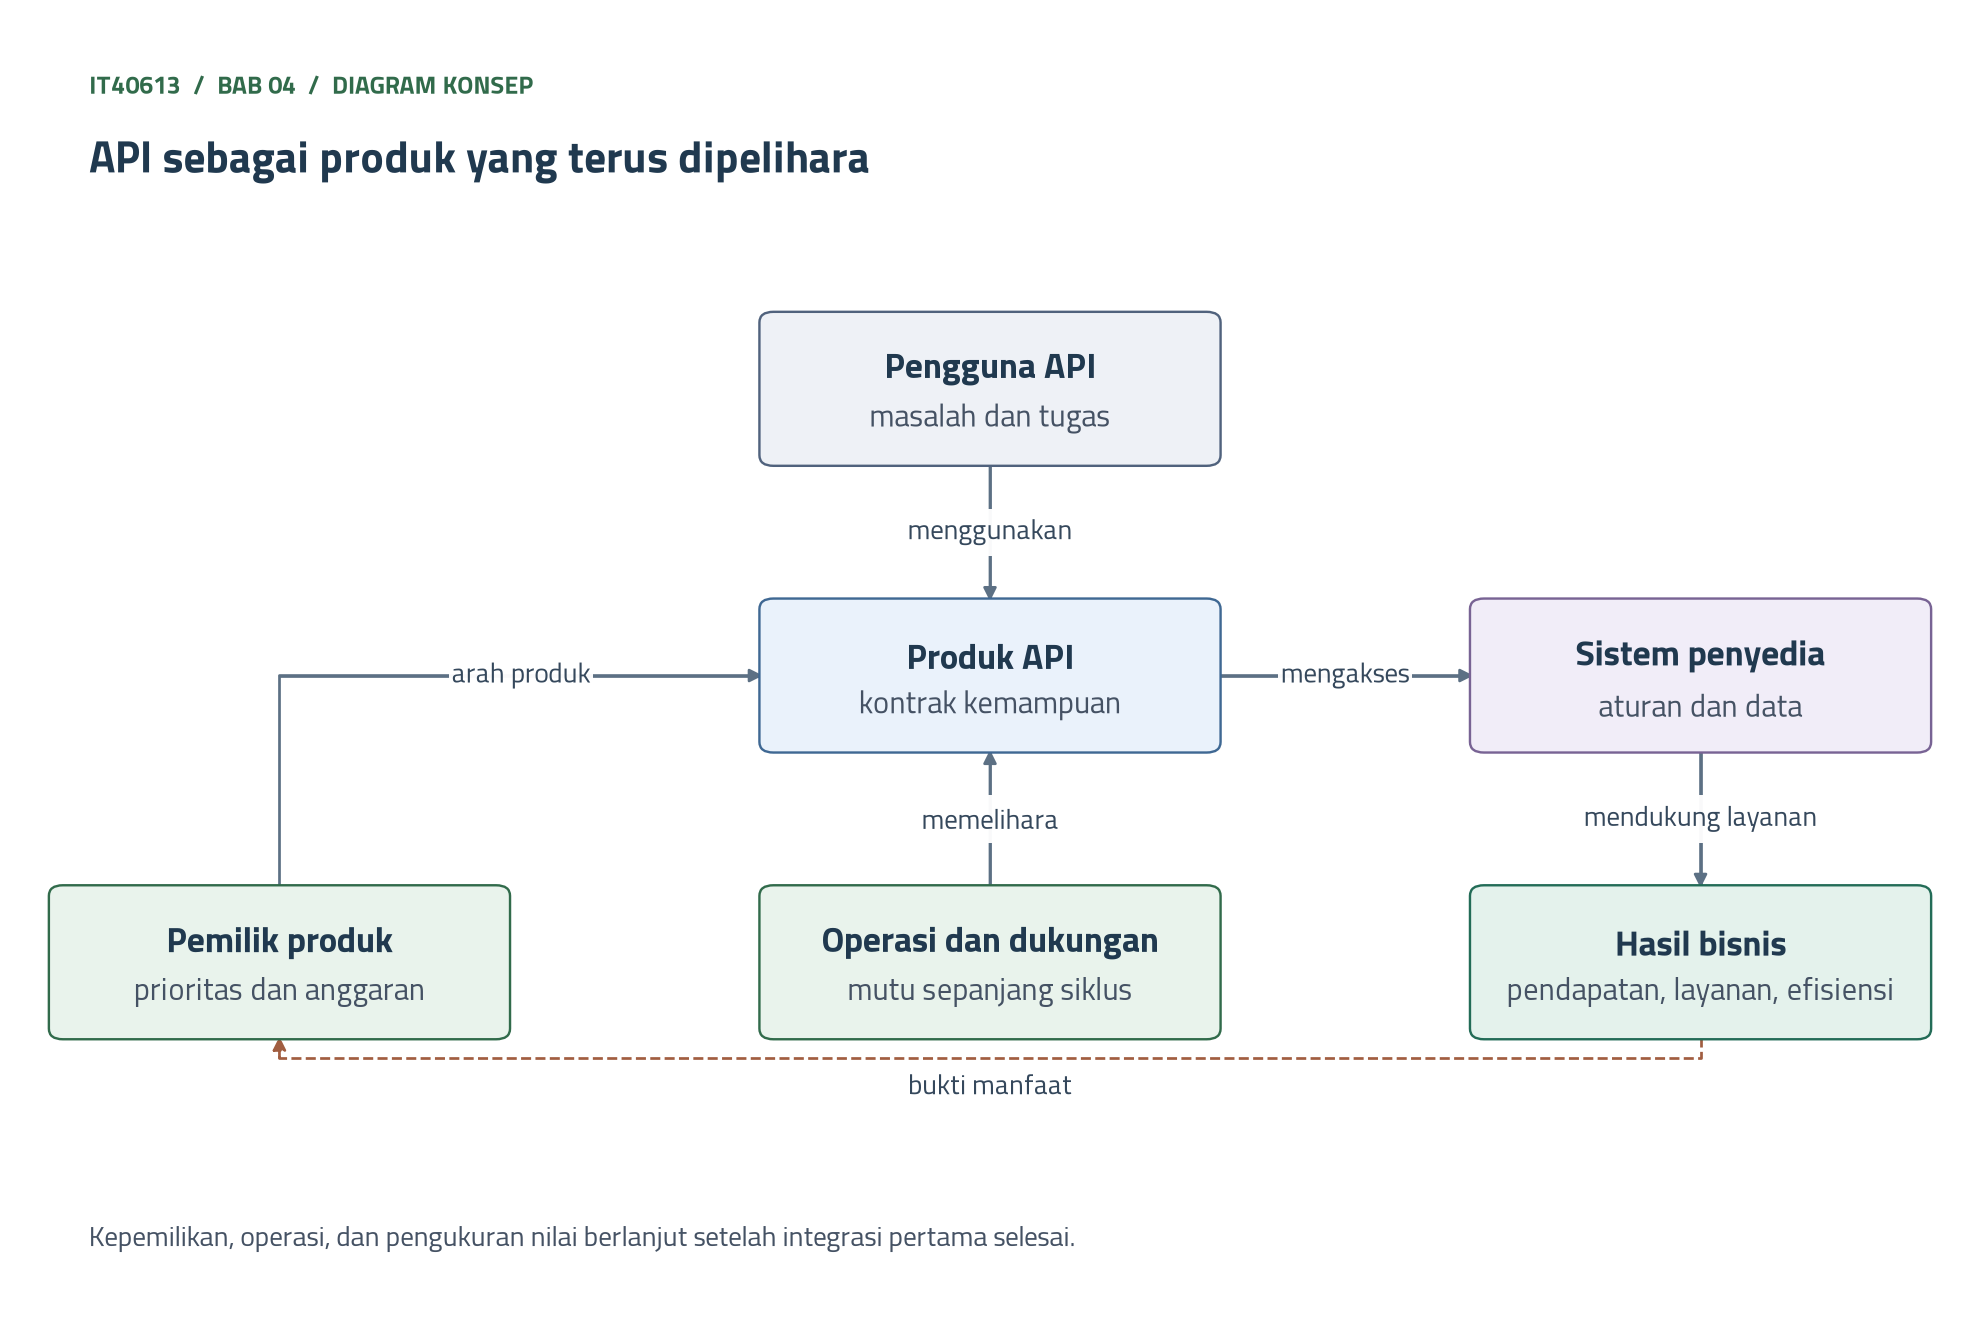
\includegraphics[width=0.96\textwidth,height=0.77\textheight,keepaspectratio]{../../figures/ch04-diagram-konsep.png}
\end{frame}

\section{Ekonomi API}

\begin{frame}{\hfill}
  \centering
  \Huge{\textbf{Ekonomi API dan\\Batas Perusahaan}}
\end{frame}

\begin{frame}{{\Large Apa Itu Ekonomi API}}
  \vspace{10pt}
  \begin{itemize}
    \item Pertukaran nilai ketika kemampuan bisnis dipakai pihak lain lewat antarmuka terkelola.
    \item Nilainya: pendapatan, biaya koordinasi yang turun, dan layanan baru.
    \item Coase: perusahaan membesar sampai biaya di dalam sama dengan biaya lewat pasar.
    \item Parker dkk.: pengembang dapat membalikkan perusahaan, nilai berpindah ke luar.
    \item Rumah sakit tidak terbalik penuh: layanan klinis inti tetap di dalam.
  \end{itemize}
  \vspace{6pt}
  {\small Analogi: warung melepas sambal dan es batu begitu pemasok tepat waktu.}
\end{frame}

\begin{frame}{{\Large API Menurunkan Biaya Melintasi Batas}}
  \centering
  \eadiagram{../../figures/ch04-batas-perusahaan.tex}
\end{frame}

\begin{frame}{{\Large Dua Contoh Berangka dan Satu Kekeliruan}}
  \vspace{10pt}
  \begin{itemize}
    \item Misalkan 6 menit per hasil: 1.100 pemeriksaan menjadi 110 jam per bulan.
    \item Misalkan Rp60.000 per jam: Rp79,2 juta per tahun, tidak pernah tampak di kontrak.
    \item Misalkan 400 telepon berkurang: 40 jam per bulan, atau Rp28,8 juta per tahun.
    \item Volume bukan nilai: misalkan panggilan naik dari 84.000 menjadi 168.000.
    \item Janji temu tetap 28.000: tiga menjadi enam panggilan, periksa \textit{error}.
  \end{itemize}
\end{frame}

\begin{frame}{{\Large Membaca Riset dan Laporan Industri}}
  \footnotesize
  \begin{tabularx}{\textwidth}{>{\raggedright\arraybackslash}p{2.2cm}
      >{\raggedright\arraybackslash}X >{\raggedright\arraybackslash}X}
    \hline
    \textbf{Sumber} & \textbf{Temuan} & \textbf{Batas pembacaan} \\ \hline
    Benzell dkk.\ 2024 & Tambahan 38,7 persen selama 16 tahun bagi pengadopsi API publik; API internal tidak berefek signifikan; risiko kebocoran naik & Perusahaan tercatat di bursa; didanai sebagian oleh dua perusahaan alat API \\ \hline
    Postman 2025 & 82 persen \textit{API-first} pada tingkat tertentu, 25 persen sepenuhnya; 65 persen memperoleh pendapatan dari API & Lebih dari 5.700 responden, 73 persen dari rekayasa perangkat lunak \\ \hline
    MuleSoft 2025 & Rata-rata 897 aplikasi, 29 persen terintegrasi; 40 persen menyebut porsi pendapatan signifikan & Lebih dari 1.050 pemimpin teknologi informasi; penerbit menjual integrasi \\ \hline
  \end{tabularx}

  \vspace{6pt}
  \small Tanyakan: siapa penerbit, siapa responden, apa yang diukur, dapatkah dipindahkan?
\end{frame}

\section{API sebagai Produk}

\begin{frame}{\hfill}
  \centering
  \Huge{\textbf{API sebagai Produk}}
\end{frame}

\begin{frame}{{\Large Apa Itu API sebagai Produk}}
  \vspace{10pt}
  \begin{itemize}
    \item API layak mendapat riset pengguna, prototipe, pengujian, dan pemeliharaan jangka panjang.
    \item Tiga kewajiban: mengenal audiens, menyelesaikan masalahnya, memperhatikan masukannya.
    \item Proyek dibatasi lingkup dan tanggal selesai; tanggung jawab produk berlanjut.
    \item Tiga pertanyaan uji: siapa penggunanya, nilai apa yang terukur, siapa pemiliknya?
    \item API internal juga produk, dengan investasi yang lebih kecil.
  \end{itemize}
  \vspace{6pt}
  {\small Analogi: kontraktor dapur pulang, pemilik restoran masih menjaga menu dan mutu.}
\end{frame}

\begin{frame}{{\Large Proyek dan Produk Setelah Serah Terima}}
  \footnotesize
  \begin{tabularx}{\textwidth}{>{\raggedright\arraybackslash}p{2.6cm}
      >{\raggedright\arraybackslash}X >{\raggedright\arraybackslash}X}
    \hline
    \textbf{Ciri} & \textbf{API sebagai proyek} & \textbf{API sebagai produk} \\ \hline
    Ukuran berhasil & Diserahkan tepat waktu dan sesuai lingkup & Masalah pengguna berkurang, terbaca dari data \\ \hline
    Akhir pekerjaan & Tanggal selesai di kontrak & Berlanjut sampai API dipensiunkan \\ \hline
    Pemilik & Manajer proyek, sampai serah terima & Pemilik produk, menetapkan prioritas dan anggaran \\ \hline
    Anggaran & Sekali bayar, perubahan menjadi permintaan baru & Tahunan, perubahan sudah direncanakan \\ \hline
    Pengguna & Disebut di dokumen kebutuhan & Dikenal, diwawancarai, dipantau pemakaiannya \\ \hline
    Dukungan & Garansi vendor dalam jangka waktu tertentu & Dokumentasi dan jalur bantuan yang terus dirawat \\ \hline
  \end{tabularx}
\end{frame}

\begin{frame}{{\Large Alur Proyek dan Siklus Hidup Produk}}
  \centering
  \eadiagram{../../figures/ch04-proyek-produk.tex}
\end{frame}

\begin{frame}{{\Large Contoh Berangka: API Klaim Tiga Tahun}}
  \vspace{10pt}
  \begin{itemize}
    \item Misalkan dibangun Rp250 juta; 9 asuransi mengubah aturan dua kali setahun: 18 perubahan.
    \item Sebagai proyek: Rp8 juta per perubahan, atau Rp144 juta per tahun. Tiga tahun: Rp682 juta.
    \item Sebagai produk: Rp180 juta per tahun. Tiga tahun: Rp790 juta, lebih mahal Rp108 juta.
    \item Misalkan penolakan turun dari 6 ke 2 persen: 468 menjadi 156 klaim per bulan.
    \item Hemat 78 jam per bulan, atau Rp168,48 juta dalam tiga tahun.
  \end{itemize}
\end{frame}

\begin{frame}{{\Large Kasus Medikara: Tiga Calon Produk API Mitra}}
  \scriptsize
  \begin{tabularx}{\textwidth}{>{\raggedright\arraybackslash}p{2.0cm}
      >{\raggedright\arraybackslash}X >{\raggedright\arraybackslash}p{1.6cm}
      >{\raggedright\arraybackslash}X >{\raggedright\arraybackslash}p{2.1cm}}
    \hline
    \textbf{Sambungan} & \textbf{Pengguna dan tugas} & \textbf{Beban manual} & \textbf{Ukuran nilai} & \textbf{Pemilik} \\ \hline
    Hasil pemeriksaan & Petugas laboratorium dan dokter: hasil benar sampai ke rekam medis & 110 jam per bulan & Waktu sampai hasil terbaca, jumlah koreksi & Manajer Laboratorium \\ \hline
    Klaim asuransi & Petugas klaim: klaim diterima pada pengiriman pertama & 117 jam per bulan & Persen klaim ditolak karena format & Manajer Klaim \\ \hline
    Rekap perusahaan & Bagian kepegawaian klien: tahu pemakaian tanpa data perorangan & 32 jam per bulan & Hari sampai rekap diterima, rekap di surel & Manajer Layanan Perusahaan \\ \hline
  \end{tabularx}

  \vspace{6pt}
  \small Total 259 jam per bulan, atau Rp186,48 juta per tahun. Urutannya mengikuti akibat bagi pengguna.
\end{frame}

\begin{frame}{{\Large Pendekatan API-first}}
  \vspace{10pt}
  \begin{itemize}
    \item Kontrak dipikirkan sejak awal, bukan ditambahkan setelah aplikasi jadi.
    \item Postman: 82 persen pada tingkat tertentu, hanya 25 persen sepenuhnya.
    \item Misalkan nama kolom keliru: 2 jam saat kontrak ditinjau, 160 jam setelah 40 klinik terhubung.
    \item Misalkan kerja berurutan 16 minggu; kontrak di awal membuatnya 12 minggu.
    \item Bukan berarti semua harus API: unggah berkas bulanan tetap masuk akal.
  \end{itemize}
  \vspace{6pt}
  {\small Analogi: memindahkan pintu di denah lebih murah daripada membongkar tembok.}
\end{frame}

\section{Audiens API}

\begin{frame}{\hfill}
  \centering
  \Huge{\textbf{Audiens API: Privat,\\Mitra, dan Publik}}
\end{frame}

\begin{frame}{{\Large Tiga Audiens, Tiga Hubungan}}
  \footnotesize
  \begin{tabularx}{\textwidth}{>{\raggedright\arraybackslash}p{2.9cm}
      >{\raggedright\arraybackslash}X >{\raggedright\arraybackslash}X >{\raggedright\arraybackslash}X}
    \hline
    \textbf{Aspek} & \textbf{Privat} & \textbf{Mitra} & \textbf{Publik} \\ \hline
    Pemanggil & Tim dan aplikasi sendiri & Pihak yang disepakati & Pihak yang belum tentu dikenal \\ \hline
    Dasar hubungan & Aturan internal & Perjanjian dan hak akses & Syarat penggunaan \\ \hline
    Pemberitahuan perubahan & Rapat antartim, cepat & Masa transisi disepakati & Panjang, pemanggil tidak dapat dihubungi satu per satu \\ \hline
    Ukuran nilai & Biaya dan waktu kerja & Layanan bersama selesai & Jangkauan dan pemakaian \\ \hline
    Tangga Bab 3 & Di luar tangga & Tingkat 1 sampai 3 & Tingkat 0 \\ \hline
    Contoh Medikara & Jadwal bagi Medikara+ & Klaim, hasil, rekap & Pencarian jadwal \\ \hline
  \end{tabularx}
\end{frame}

\begin{frame}{{\Large Audiens dan Kepekaan Data}}
  \centering
  \eadiagram{../../figures/ch04-audiens-sensitivitas.tex}
\end{frame}

\begin{frame}{{\Large Contoh Berangka dan Kasus Jadwal}}
  \vspace{10pt}
  \begin{itemize}
    \item Publik: tanpa akun, 1.000 panggilan per hari, tanpa data pasien.
    \item Mitra: 300 panggilan per hari per klinik, 12.000 untuk 40 klinik.
    \item Privat: misalkan vendor membaca 140 tabel, butuh 2, risiko 138.
    \item Kasus: jadwal yang sama tampil dalam tiga bentuk, pemiliknya satu.
    \item Akibatnya vendor Medikara+ harus mengubah aplikasinya.
  \end{itemize}
  \vspace{6pt}
  {\small Publik tidak berarti tanpa autentikasi atau bebas biaya.}
\end{frame}

\section{Point-to-Point dan Utang Integrasi}

\begin{frame}{\hfill}
  \centering
  \Huge{\textbf{Point-to-Point dan\\Utang Integrasi}}
\end{frame}

\begin{frame}{{\Large Dari Batas Rumus ke Sambungan yang Berjalan}}
  \vspace{10pt}
  \begin{itemize}
    \item Sembilan sistem: batas $n(n-1)/2$ adalah 36 pasangan, bukan anggaran.
    \item Lima SIMRS dan empat tujuan yang berjalan: 20 sambungan.
    \item Misalkan Rp45 juta per sambungan: Rp900 juta per tahun.
    \item Satu tujuan baru berarti 5 sambungan baru, atau tambah Rp225 juta per tahun.
    \item Misalkan 4 pembaruan spesifikasi di 5 tempat: 20 pekerjaan, Rp240 juta per tahun.
  \end{itemize}
  \vspace{6pt}
  {\small Analogi: colokan tambahan tanpa penanda membuat setiap perbaikan menjadi mahal.}
\end{frame}

\begin{frame}{{\Large Lapisan Bersama Tidak Selalu Lebih Murah}}
  \footnotesize
  \begin{tabularx}{\textwidth}{>{\raggedright\arraybackslash}p{2.0cm}
      >{\raggedright\arraybackslash}X >{\raggedright\arraybackslash}X
      >{\raggedright\arraybackslash}X >{\raggedright\arraybackslash}X}
    \hline
    \textbf{Jumlah tujuan} & \textbf{Sambungan langsung} & \textbf{Biaya langsung} & \textbf{Sambungan lewat lapisan} & \textbf{Biaya lewat lapisan} \\ \hline
    1 & 5 & Rp225 juta & 6 & Rp570 juta \\ \hline
    2 & 10 & Rp450 juta & 7 & Rp615 juta \\ \hline
    3 & 15 & Rp675 juta & 8 & Rp660 juta \\ \hline
    4 & 20 & Rp900 juta & 9 & Rp705 juta \\ \hline
    6 & 30 & Rp1,35 miliar & 11 & Rp795 juta \\ \hline
    8 & 40 & Rp1,8 miliar & 13 & Rp885 juta \\ \hline
  \end{tabularx}

  \vspace{6pt}
  \small Misalkan lapisan Rp300 juta per tahun dan satu sambungan Rp45 juta per tahun. Impas mulai tiga tujuan.
\end{frame}

\begin{frame}{{\Large Utang Integrasi: Tercatat dan Tersembunyi}}
  \centering
  \eadiagram{../../figures/ch04-utang-integrasi.tex}

  \vspace{4pt}
  {\small Biaya tersembunyi terhitung sekitar Rp497 juta per tahun, 55 persen di atas anggaran tercatat.}
\end{frame}

\begin{frame}{{\Large Kasus Medikara: Pokok dan Bunga}}
  \footnotesize
  \begin{tabularx}{\textwidth}{>{\raggedright\arraybackslash}p{2.7cm}
      >{\raggedright\arraybackslash}p{1.8cm} >{\raggedright\arraybackslash}p{2.0cm}
      >{\raggedright\arraybackslash}p{1.5cm} >{\raggedright\arraybackslash}X}
    \hline
    \textbf{Sambungan} & \textbf{Pokok} & \textbf{Bunga per tahun} & \textbf{Balik modal} & \textbf{Akibat di luar hitungan} \\ \hline
    Hasil pemeriksaan & Rp200 juta & Rp79,2 juta & 2,5 tahun & Salah ketik hasil, pasien menunggu \\ \hline
    Klaim asuransi & Rp250 juta & Rp84,24 juta & 3,0 tahun & Pembayaran klaim tertahan \\ \hline
    Rekap perusahaan & Rp150 juta & Rp23,04 juta & 6,5 tahun & Data karyawan beredar di surel \\ \hline
  \end{tabularx}

  \vspace{6pt}
  \small Pokok Rp600 juta, bunga Rp186,48 juta per tahun. Jam kerja saja tidak membenarkan API rekap.
  Hasil pemeriksaan didahulukan karena akibatnya mengenai pasien.
\end{frame}

\section{Model Bisnis}

\begin{frame}{\hfill}
  \centering
  \Huge{\textbf{Model Bisnis\\Berbasis API}}
\end{frame}

\begin{frame}{{\Large API Dijual dan API Pendukung Produk}}
  \vspace{10pt}
  \begin{itemize}
    \item Medjaoui dkk.: Stripe dan Twilio menjual kemampuan yang berdiri sendiri.
    \item Salesforce dan YouTube: API mendukung platform, sering gratis.
    \item Pada skema Bab 2, langganan Rp3 juta per bulan setara Rp400 per panggilan pada kuota 7.500.
    \item Tarif per panggilan menghukum klinik saat sistem mengulang akibat \textit{error}.
    \item API mitra Medikara mendukung layanan. Ukurannya layanan selesai, bukan pendapatan API.
  \end{itemize}
  \vspace{6pt}
  {\small Analogi: ongkir dapat dibayar pembeli, penjual, atau disubsidi dalam harga barang.}
\end{frame}

\begin{frame}{{\Large Pilihan Model Bisnis}}
  \scriptsize
  \begin{tabularx}{\textwidth}{>{\raggedright\arraybackslash}p{2.6cm}
      >{\raggedright\arraybackslash}p{2.2cm} >{\raggedright\arraybackslash}X >{\raggedright\arraybackslash}X}
    \hline
    \textbf{Model} & \textbf{Pembayar} & \textbf{Contoh} & \textbf{Dasar penilaian} \\ \hline
    Bayar per transaksi & Pemakai API & Stripe: 2,9 persen ditambah 30 sen dolar. Medikara+: Rp10.000 per verifikasi penjaminan, Rp960 juta per tahun & Pendapatan bersih per transaksi berhasil \\ \hline
    Langganan & Mitra & 40 klinik $\times$ Rp3 juta $\times$ 12 bulan = Rp1,44 miliar per tahun & Klinik aktif yang bertahan \\ \hline
    Bagian dari paket & Pembeli paket & Paket 200 karyawan Rp100 juta, Medikara menyimpan Rp10 juta & Nilai layanan selesai \\ \hline
    Investasi operasional & Organisasi sendiri & API klaim yang tidak dijual, hemat Rp56,16 juta per tahun & Biaya kerja ulang yang turun \\ \hline
    Kewajiban & Organisasi sendiri & 10 sambungan BPJS Kesehatan dan SATUSEHAT, Rp450 juta per tahun & Kepatuhan, kiriman berhasil \\ \hline
  \end{tabularx}
\end{frame}

\begin{frame}{{\Large Sektor Pembayaran dan Sektor Kesehatan}}
  \vspace{10pt}
  \begin{itemize}
    \item Stripe: transaksi 100 dolar dikenai 3,20 dolar, tanpa biaya bulanan.
    \item SNAP: standar nasional, wajib bertahap, dikelola ASPI sejak 1 September 2023.
    \item Data kesehatan bukan komoditas bebas jual: Medikara menjual layanan di sekitar data.
    \item SMART on FHIR: aplikasi medis ditulis sekali, berjalan pada berbagai sistem.
    \item Aturan Amerika Serikat membatasi biaya API bersertifikat. Pembanding, bukan aturan Indonesia.
  \end{itemize}
\end{frame}

\section{Inventaris}

\begin{frame}{\hfill}
  \centering
  \Huge{\textbf{Menyusun Inventaris\\Integrasi dan API}}
\end{frame}

\begin{frame}{{\Large Mengapa Inventaris dan Apa Isinya}}
  \vspace{10pt}
  \begin{itemize}
    \item Postman: 34 persen tidak dapat menemukan API yang sudah ada.
    \item OWASP memasukkan inventaris yang buruk ke dalam sepuluh risiko API 2023.
    \item Enam kolom wajib: asal, tujuan, data, pemilik, cara pertukaran, audiens.
    \item Kolom keputusan: volume, sambungan, peran, biaya, jam manual, status bukti.
    \item Semua integrasi dicatat, termasuk surel. Yang belum diketahui ditulis apa adanya.
  \end{itemize}
  \vspace{6pt}
  {\small Analogi: daftar aset rumah memuat lokasi, pemilik, dan kondisi, bukan hanya nama barang.}
\end{frame}

\begin{frame}{{\Large Peta Keputusan untuk Setiap Baris}}
  \centering
  \eadiagram{../../figures/ch04-peta-keputusan.tex}

  \vspace{4pt}
  {\small Tidak semua baris perlu menjadi API.}
\end{frame}

\begin{frame}{{\Large Kasus Medikara: 10 Baris, 100 Sambungan}}
  \vspace{10pt}
  \begin{itemize}
    \item 10 baris mewakili 100 sambungan. Hanya 10 sambungan memakai API resmi, milik pihak wajib. INT-03: basis data di 3 rumah sakit, API bawaan di 2.
    \item Status bukti: 7 terverifikasi, 2 wawancara, 1 belum terverifikasi.
    \item Tercatat Rp900 juta per tahun; kerja manual 357 jam per bulan, Rp257,04 juta per tahun.
    \item Keputusan: 4 calon produk, 4 dirapikan, 1 dibiarkan, 1 ditelusuri.
    \item Paling mahal: 20 sambungan INT-01 sampai INT-04. Paling rawan: INT-03 dan INT-06.
  \end{itemize}
\end{frame}

\section{Aktivitas}

\begin{frame}{{\Large Aktivitas: Peran dan Langkah Kerja}}
  \vspace{6pt}
  \begin{itemize}
    \item Anggota non-teknis mewawancarai pemilik proses: kegunaan dan masalah tiap integrasi.
    \item Anggota teknis menelusuri dokumentasi, konfigurasi, atau kontrak vendor.
    \item Isi kolom wajib, tandai status bukti, pisahkan biaya terukur dari perkiraan.
    \item Lewatkan setiap baris pada peta keputusan.
    \item Pilih tiga integrasi berisiko untuk Bab 5 sampai Bab 7.
  \end{itemize}
  \vspace{4pt}
  {\small Berkas: \berkas{sources/chapter04/}. Data pribadi pasien dan karyawan tidak boleh dimasukkan.}
\end{frame}

\begin{frame}{{\Large Aktivitas: Luaran dan Kriteria}}
  \footnotesize
  \begin{tabularx}{\textwidth}{>{\raggedright\arraybackslash}X r}
    \hline
    \textbf{Kriteria} & \textbf{Bobot} \\ \hline
    Ketepatan konsep: audiens, produk dan proyek, serta utang integrasi & 25\% \\ \hline
    Keterlacakan bukti: fakta, asumsi, dan perkiraan dibedakan dan punya sumber & 30\% \\ \hline
    Alasan keputusan dan pengorbanan: integrasi mahal atau rawan dipilih dengan alasan terukur & 30\% \\ \hline
    Keterbacaan artefak: dipahami pembaca yang tidak ikut menyusun & 15\% \\ \hline
  \end{tabularx}

  \vspace{8pt}
  \small Luaran untuk C2: inventaris integrasi dan API, ditambah catatan integrasi paling mahal atau paling rawan.
  Pendalaman opsional: membaca katalog SNAP Developer Site milik ASPI.
\end{frame}

\section{Ringkasan dan Latihan}

\begin{frame}{{\Large Ringkasan}}
  \vspace{10pt}
  \begin{itemize}
    \item API menurunkan biaya melintasi batas perusahaan; volume panggilan bukan ukuran nilai.
    \item Produk punya pengguna, pemilik, ukuran, dan anggaran setelah serah terima.
    \item Audiens berbeda dari kepekaan data. Lokasi internal tidak menjamin hak akses.
    \item Rp900 juta tercatat, sekitar Rp497 juta tersembunyi. Lapisan bersama impas mulai tiga tujuan.
    \item API tanpa pemilik akan kembali menjadi proyek berikutnya.
  \end{itemize}
\end{frame}

\begin{frame}{{\Large Latihan}}
  \vspace{10pt}
  \begin{enumerate}
    \item Jelaskan dengan contoh mengapa integrasi \textit{point-to-point} yang jumlahnya terus bertambah menaikkan biaya organisasi.
    \item Tentukan apakah API pendaftaran pasien Medikara sebaiknya privat, mitra, atau publik, lalu tuliskan alasannya.
    \item Sebutkan tiga ciri yang membedakan API yang dikelola sebagai produk dari API yang dibangun sebagai proyek sekali jadi.
  \end{enumerate}
\end{frame}

\end{document}
